%!TEX root = proposal.tex

Our static analysis techniques for Bloom can
%conservatively 
affirm that a given program has eventually consistent outcomes.
If the analysis is unable to do so---due to the presence of non-monotonic deductions
that follow asynchronous communication---a dataflow visualization tool can display the
program locations where coordination may need to be added to ``guard'' the
non-monotonic operations.  
Figure~\ref{fig:kvs} shows a Bloom implementation of a simple key-value store
and its accompanying dataflow visualization.  Note the white circles on the edges leading
into the \texttt{kvstate} collection, indicating non-monotonic operations corresponding to 
the deletion in lines~\ref{line:bloom-kvs-del1} and~\ref{line:bloom-kvs-del2}; clicking on those circles brings up the relevant non-monotonic statements.


\begin{figure}[t]
\begin{minipage}{.48\textwidth}

\begin{scriptsize}
\begin{lstlisting}
module KVSProtocol
  state do
    interface input, :kvput, [:client, :key] => [:reqid, :value]
    interface input, :kvdel, [:key] => [:reqid]
    interface input, :kvget, [:reqid] => [:key]
    interface output, :kvget_response, [:reqid] => [:key, :value]
  end
end

module BasicKVS
  include KVSProtocol

  state do
    table :kvstate, [:key] => [:value]
  end

  bloom :mutate do
    kvstate <+ kvput {|s| [s.key, s.value]}
    kvstate <- (kvstate * kvput).lefts(:key => :key) (*\label{line:bloom-kvs-del1}*)
    kvstate <- (kvstate * kvdel).lefts(:key => :key) (*\label{line:bloom-kvs-del2}*)
  end

  bloom :get do
    temp :getj <= (kvget * kvstate).pairs(:key => :key)
    kvget_response <= getj do |g, t|
      [g.reqid, t.key, t.value]
    end
  end

end

\end{lstlisting}
\end{scriptsize}
\end{minipage}
\begin{minipage}{.48\textwidth}
\raggedleft
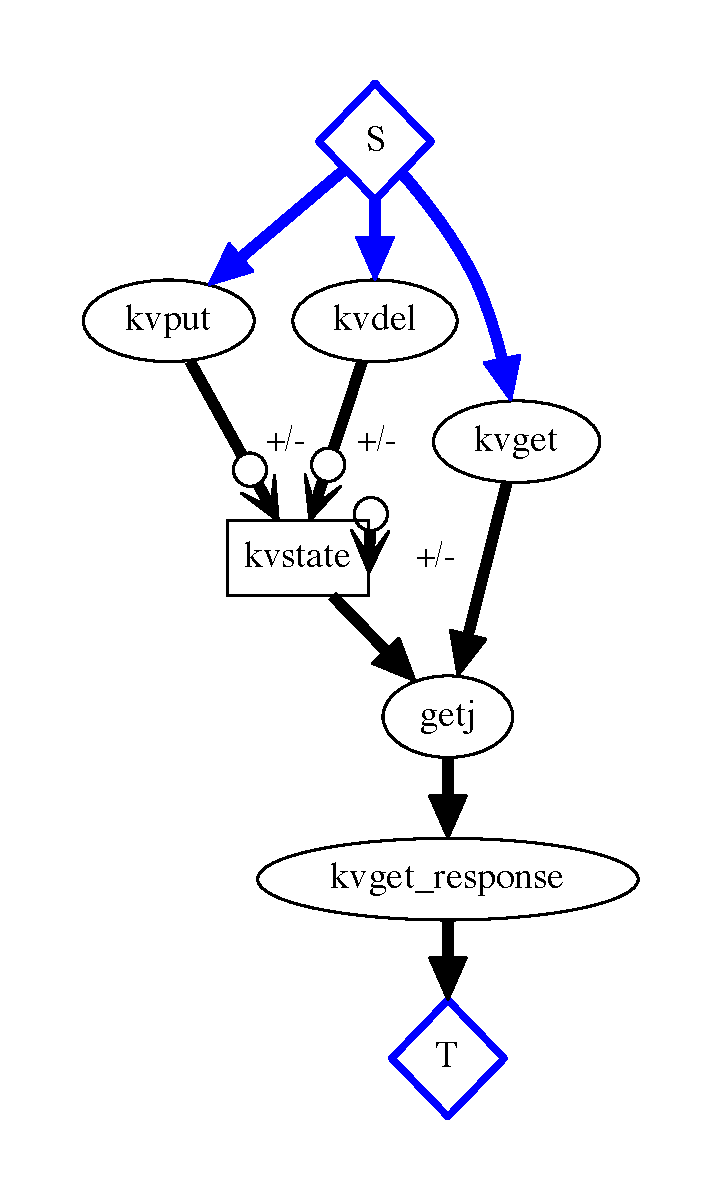
\includegraphics[width=0.7\linewidth]{kvs.pdf}
\end{minipage}

\vspace{-10pt}
\caption{A Bloom key-value store and its CALM visualization}
\label{fig:kvs}
\vspace{-2pt}

\end{figure}

The interface presents a visualization of the static dataflow analysis that we perform on a Bloom program.  While useful, such visualizations do not scale well to large programs and big graphs. Moreover, in many cases a programmer does not want to see this level of detail for all the code in their program.  For instance, when using encapsulated library modules, it is helpful to reason only about their interfaces, not their internals.  Ideally, CALM analysis should be encapsulated via annotations on a module's external input/output API, exposing only the consistency implications of composing the module with other code.

\begin{figure}[t]
\begin{minipage}{.63\textwidth}
\footnotesize

%%\centering
\begin{tabular}{|l|l|p{7cm}|}
\hline
Class & Label & Interpretation \\ \hline
Primitive & $\bot$ & Transformation does not affect consistency \\ \cline{2-3}
& $N$ & Non-monotonic (order-sensitive) transformation \\ \cline{2-3}
& $A$ & Asynchronous (unordered) communication \\ \hline
Compound & $D$ & Diffluent (non-confluent): non-deterministic results across executions or replicas \\ \cline{2-3}
& $R$ & Restores order.  Represents some coordination protocol. \\ \hline

\end{tabular}

%\vspace{-10pt}
%\caption{Consistency Labels}
%\label{fig:basic-labels}
%\vspace{-2pt}
%\end{figure}


%\begin{figure}[t]

\end{minipage}
\begin{minipage}{.35\textwidth}
\raggedleft

\footnotesize
\begin{tabular}{|l|p{4cm}|}
\hline
Rule & Interpretation \\ \hline
$\alpha\alpha \rightarrow \alpha$ & label repetition does not change semantics \\ \hline
$\bot \beta \rightarrow \beta$ & $\bot$ has no effect on neighboring \\
$\beta \bot \rightarrow \beta$ & labels\\ \hline
$AN \rightarrow D$ & Loss of order followed by order-sensitivity causes diffluence \\ \hline
$D \alpha \rightarrow D$ & \\
$\alpha D \rightarrow D$ & Once diffluent, always diffluent\\ \hline
$AR \rightarrow R$ & Order lost and regained \\ \hline
$RA \rightarrow A$ & Order imposed and then lost \\ \hline
$RN \rightarrow R$ & $N$ does no harm to $R$ flows \\ \hline
$NR \rightarrow N$ & $R$ does no good for $N$ flows \\ \hline

\end{tabular}
\end{minipage}
\caption{Labels and Reduction Rules \jmh{what is the distinction between $\alpha$ and $\beta$ and did I use them right?}}
\label{fig:rules}
\end{figure}

To summarize the input-to-output relationships in a module, we have to characterize the dataflow \emph{paths} from each of its input interfaces to each of its output interfaces.  We do this by (1) labeling individual edges of a dataflow graph like Figure~\ref{fig:kvs} with certain properties, and (2) understanding the transitive implications of these properties across multiple edges.  The left side of Figure~\ref{fig:rules} shows the labels that the analysis assigns to individual edges (``primitive''), and the labels that arise via dataflow composition (``compound'') as described in the rules on the right side of Figure~\ref{fig:rules}.  

As an illustration, consider again the overwriting key-value store presented in Figure~\ref{fig:kvs}.
CALM analysis detected a non-monotonic operation in the dataflow edge from \texttt{kvput} to \texttt{kvstate}: the appearance of PUT requests contribute to the deletion of old values (line~\ref{line:bloom-kvs-del1}).  Thus we label that edge with an $N$.  The other edge labels in Figure~\ref{fig:kvs} are either $N$ or $\bot$, so as we transitively combine edges, the first two rules on the right side of Figure~\ref{fig:rules} lead us to associate with BasicKVS the following signature for the single output interface and two input interfaces:
$kvget\_response: \{N(put) \; | \; \bot(get)\}$.  

Consider now a larger system that uses this key-value store as a component.  It will not be safe to attach an asynchronous ($A$)
stream to the \texttt{kvput} interface of the store, as this will lead to a diffluent ($D$) consistency label
(due to the rule $AN \rightarrow D$).  For asynchronous ($A$) inputs to this module,
order must be \emph{restored} (via
interposition of a dataflow labeled $R$) 
before composing with \texttt{kvput}.  This corresponds to intuition:
a key-value store with ``last writer wins'' semantics like Figure~\ref{fig:kvs} is clearly sensitive to the order in which it receives writes.
If the KVS is replicated, we must be careful about write reordering in the network, as this
may lead to inconsistent state on different replicas.
Reads, on the other hand, may be reordered freely.

\subsection{Widespread CALM Analysis: Service Composition}
The analysis framework above is helpful for analyzing pure Bloom programs that span multiple modules.
In practice, however, many distributed applications are not written in any single language, nor are all their components available for deep analysis.  Instead, many systems are compositions of large distributed services, loosely coupled using message-based APIs.
Such services are often implemented in a variety of programming 
languages, and in some cases they are opaque and outside the control of
the programmer using them.  
Many services (e.g. data stores and message queues) provide their own 
consistency guarantees, but how are we to reason about the consistency of an end-to-end
\emph{application} that calls out to various such services and transforms
and combines their responses?  

% We believe that the intuitions behind the CALM Theorem should apply at this level of reasoning,
% just as they applied to the low-level composition of operators
% in a Bloom execution.  We envision a scenario where Bloom is used as an \emph{orchestration} language for composing applications from multiple services.  The ``primitive'' consistency properties of many services in wide use today are well-known: for example, there are various libraries for distributed consensus that could be labeled $R$, there are various libraries for order-insensitive key-value stores that could be labeled $\bot$, and so on.  

% Consider an inventory management application 
% that makes calls into two asynchronously updated but
% eventually consistent datastores.  It selects from the first service---an 
% inventory datastore---the model numbers of all toaster ovens that are currently in stock.  For each, it probes the second datastore---a recall database---to
% see if the unit has been recalled.  Finally, the application returns the 
% set of model numbers for units that have \emph{not} been recalled.  Observe that this
% application has a race condition due to the negation (``not recalled''): for a given model number $N$, the order of a request to lookup $N$ and a request to insert a recall for $N$ will determine whether or not the system returns $N$.  In a distributed implementation, both orderings could occur at different replicas, yielding inconsistent results.  
% If the orchestration
% application that correlates the results from the different datastores were written in Bloom, we would observe that although the datastores are monotonic, 
% the manner in which their results are \emph{used} is not.  If the inputs to 
% the datastores are asynchronous (reorderable), then the output of the 
% application may be inconsistent.  In the Bloom labeling system presented above, both services would be labeled 
% $A$---that is, asynchronously updated but otherwise monotonic.  The orchestration code that connects them would be 
% labeled $N$---non-monotonic, due to the negation.  The resulting composition would then be labeled $D$---divergent, with
% a point of order in the orchestration code that should be resolved (e.g., by versioning the recall database and issuing queries against the 
% oldest ``complete'' version).
% 
% 
% \jmh{Make an explicit plan here to do something new with widely used systems -- zookeeper+voldemort+something?  Perhaps talk about potential collaboration with LinkedIn.}

The labeling system presented above provides a framework for reasoning about service composition that is 
mostly independent of Bloom, so long as we can accurately attribute consistency labels to service APIs.
If the services are written in Bloom, we can derive their labels automatically---otherwise we may rely on annotations.
As the example above indicated, however, we must be very careful how we \emph{use} data returned from 
eventually consistent services
if we wish to assert that application output is likewise consistent.  Hence the ``glue'' or ``orchestration'' language used
to compose services must also be amenable to CALM analysis and label propagation.  Bloom is our exemplar of such a language.

\subsection{Summary of Tasks and Goals}
\begin{itemize}
\item \textbf{Path labeling and label propagation:}
The framework of labels and rules in Figure~\ref{fig:rules} is not yet complete; we are still formalizing its theory to prove correctness, and developing the program analysis tools to automatically label code written in Bloom and \blooml.  The labeling technique should be a confluent term rewriting system, allowing us to 
characterize any dataflow as a compact expression with an intuitive 
meaning in the context of distributed systems.

\item \textbf{Automated coordination synthesis:}
  Programs that use non-monotonic constructs without coordination may produce
  non-deterministic behavior. We are exploring how such programs might be
  \emph{automatically} enhanced with order-restoring coordination mechanisms
  ($R$) to achieve consistency. We envision providing a library of built-in
  coordination strategies (e.g., Paxos, totally ordered broadcast, ordered
  unicast), and also allowing programmers to provide their own protocols. It
  seems clear that a general-purpose, heavyweight coordination protocol (e.g., Paxos)
  may be interposed at arbitrary ``points of order'' to ensure that all nodes
  agree on a message order.  More interestingly, we would like to automatically
  discover cases where more efficient but more limited protocols---e.g.,
  ordered unicast delivery between pairs of nodes---are sufficient to ensure consistency.
  We could then search the space of points-of-order and coordination protocols
  to select the most efficient coordination strategy.

\item \textbf{Uniform error communication and handling:}
  A significant challenge for an orchestration language is to provide robust
  error handling. Calls to services can fail in many different ways. In some
  cases services can report the error back to the caller along with relevant
  information about its cause, while in other cases applications must manage
  timeout and retry logic.  Since a robust orchestration language will be
  fundamentally non-deterministic, we will have to revisit the consistency
  labeling system to accommodate this uncertainty.

\item \textbf{Evaluation:} As a proof of concept, we intend to implement a
  collection of services and applications for a social network.  We are currently
  collaborating with engineers at LinkedIn and plan to either emulate or
  integrate with their architecture, which employs a deeply service-oriented design.  We hope to show how CALM analysis can ease the burden of reasoning
  about the behavior of applications that call out to a number of services
  (including data stores, message queues, coordination services like Zookeeper,
  and logging subsystems) with different service-level consistency guarantees.

\end{itemize}

